To study excited \cascade baryons the simulation of signal events is needed.
For this study 1.5 million signal events have been generated.
The decay channel for the simulation is shown in figure \ref{fig:eventgeneration_decaychannel}. 

\begin{figure}[htbp]
	\centering
			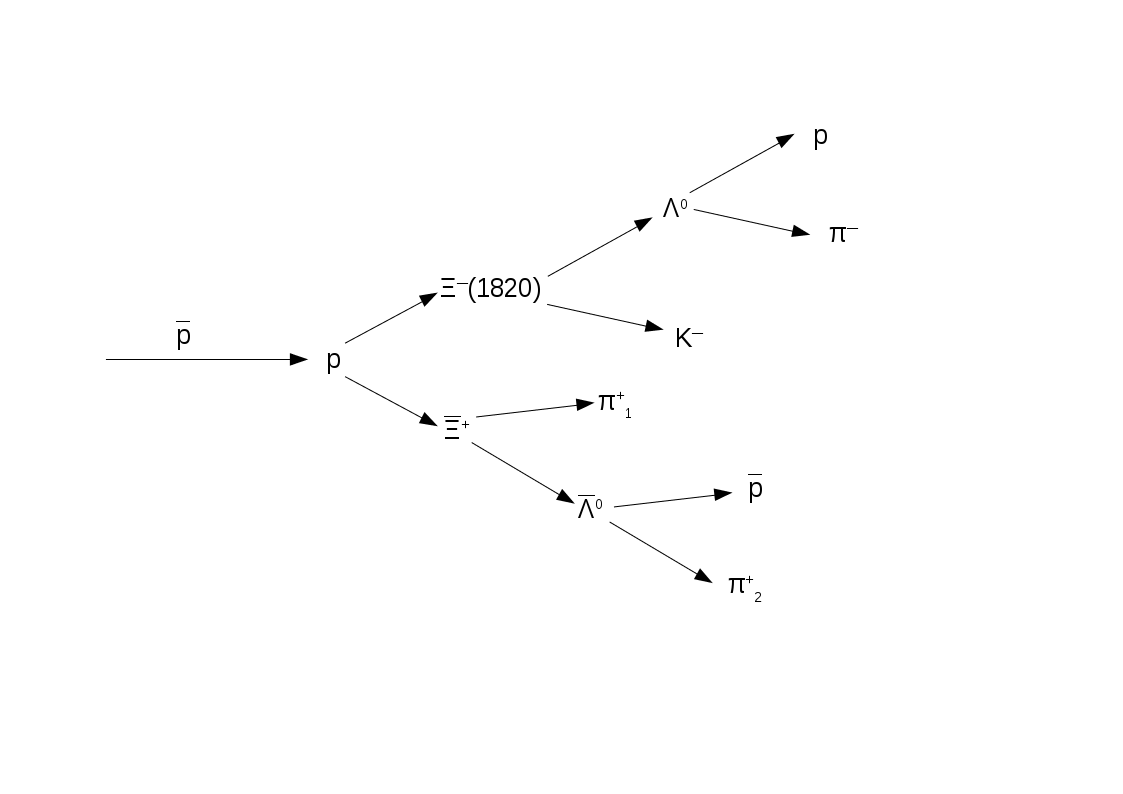
\includegraphics[width=1.00\textwidth]{./plots/DecayChannelXi1820.png}
	\caption{Simulated decay channel}
	\label{fig:eventgeneration_decaychannel}
\end{figure}

For the charge conjungated channel were also 1.5 million signal events generated.
The parameter which are used for the event generation are shown in table \ref{tab:eventgeneration_parameter}.

\begin{table}[htbp]
	\caption{Parameter for event generation}
	\label{tab:eventgeneration_parameter}
	\centering
	\begin{tabular}{ll}
		\hline
		Parameter & Value \\
		\hline
		\hline
		Beam momentum & 4.6 \massunit \\
		Production & PHSP \\
		Tracking & Ideal \\
		Particle ID & Ideal \\\hline
		 
	\end{tabular}
\end{table}

The chosen beam momentum value is 100 MeV over the production threshold of \excitedcascade and \anticascade.
The production cross section is expected to be of the same order ($\sim \mu\unit{b}$) as for \cascade \cite{PANDAphysics2009}.\\
\vspace{11pt} 

The used software versions for Pandaroot and the external software is listed in table \ref{tab:eventgeneration_software} 

\begin{table}[htb]
	\centering
	\caption{Used software versions}
	\label{tab:eventgeneration_software}
	\begin{tabular}{ll}
		\hline
		Software & Version \\
		\hline
		\hline
		FairSoft & mar15\\
		FairRoot & v-15.03a \\
		PandaRoot & trunk revision 28555 \\
		Geant & 3\\
		Genfit & 1\\\hline
			 
	\end{tabular}
\end{table}


The \excitedcascade was not defined in the evt.pdl file. 
The Lines in the code sniplet \ref{lst:eventgeneration_evtpdl} shown how the particle was added to the file.
As the properties of \excitedcascade I am using the values which are shown in table \ref{tab:eventgeneration_Xivalues}.
These values are taken from \cite{PDG}.

\begin{lstlisting}[caption={sniplet from evt.pdl}\label{lst:eventgeneration_evtpdl}, captionpos=t,breaklines=true]
add  p Particle Xi(1820)- 23314 1.8230000e+00 2.4000000e-02 2.0000000e-01 -3 3 0.0000000e+00 23314
add  p Particle anti-Xi(1820)+ -23314 1.8230000e+00 2.4000000e-02 2.0000000e-01 3 3 0.0000000e+00 -23314
\end{lstlisting}

\begin{table}[tb]
	\centering
	\caption{Values for \excitedcascade and \excitedanticascade from \cite{PDG}}
	\label{tab:eventgeneration_Xivalues}
	\begin{tabular}{lllllll}
		\hline
		Particle & J & I & P & Charge & Mass  & Width \\
		\hline
		\hline
		\excitedcascade & $\frac{3}{2}$ & $\frac{1}{2}$ & ($-1$) & ($-1$) & ($1.823 \pm 5$)\massunit & ($0.024 \pm 6) $ GeV \\
		\excitedanticascade & $\frac{3}{2}$ & $\frac{1}{2}$ & ($-1$) & 1 & ($1.823 \pm 5$)\massunit & ($0.024 \pm 6) $ GeV\\
		\hline
		  
	\end{tabular}
\end{table}

The generated transverse momentum against the longitudinal momentum for \lam, \alam, \anticascade and \excitedcascade is 
presented in figure \ref{fig:MC_lambda0_pt_vs_pz}% -- \ref{fig:MC_xi_pt_vs_pz}.\\


\begin{figure}
	\subfigure[\lam]{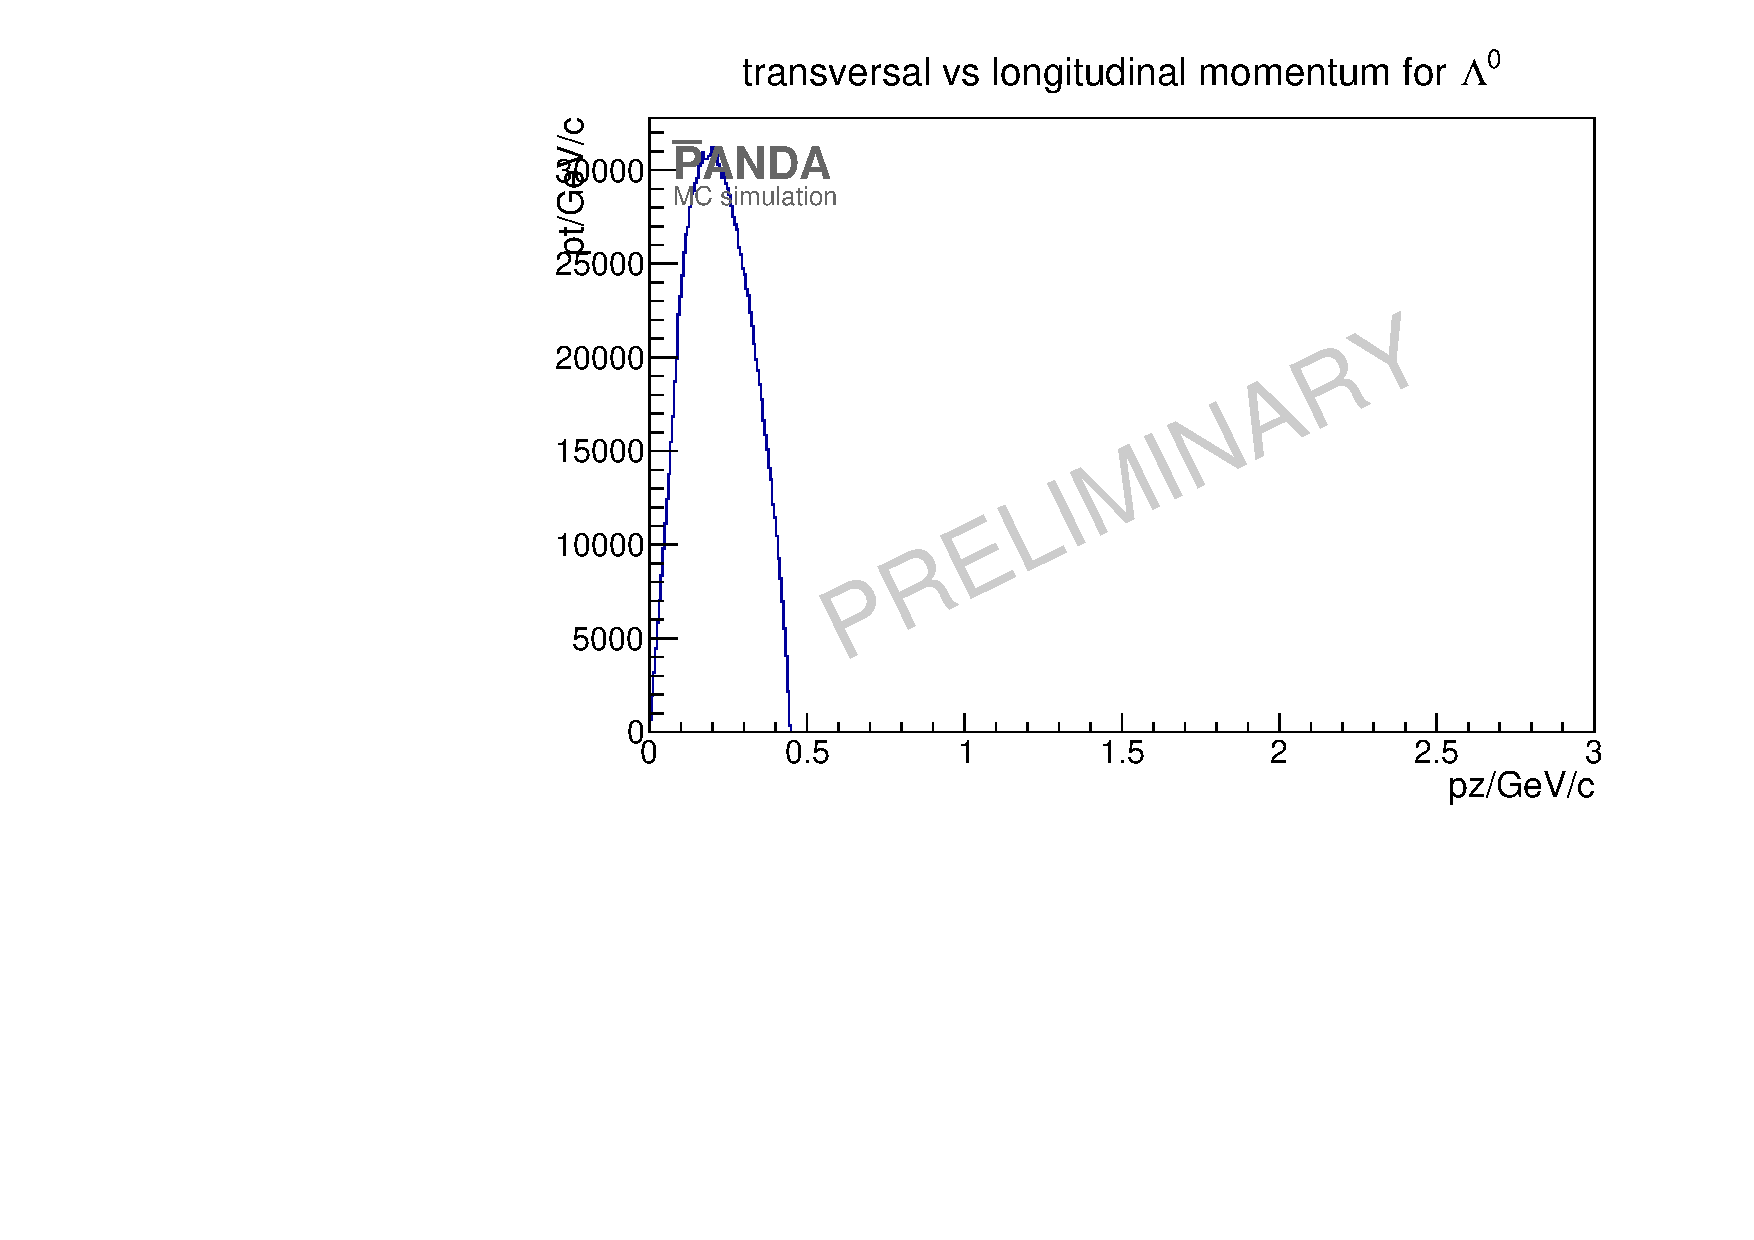
\includegraphics[width=0.49\textwidth]{./plots/lambda0/Lambda0_MC_pt_vs_pz.pdf}}
	\subfigure[\alam]{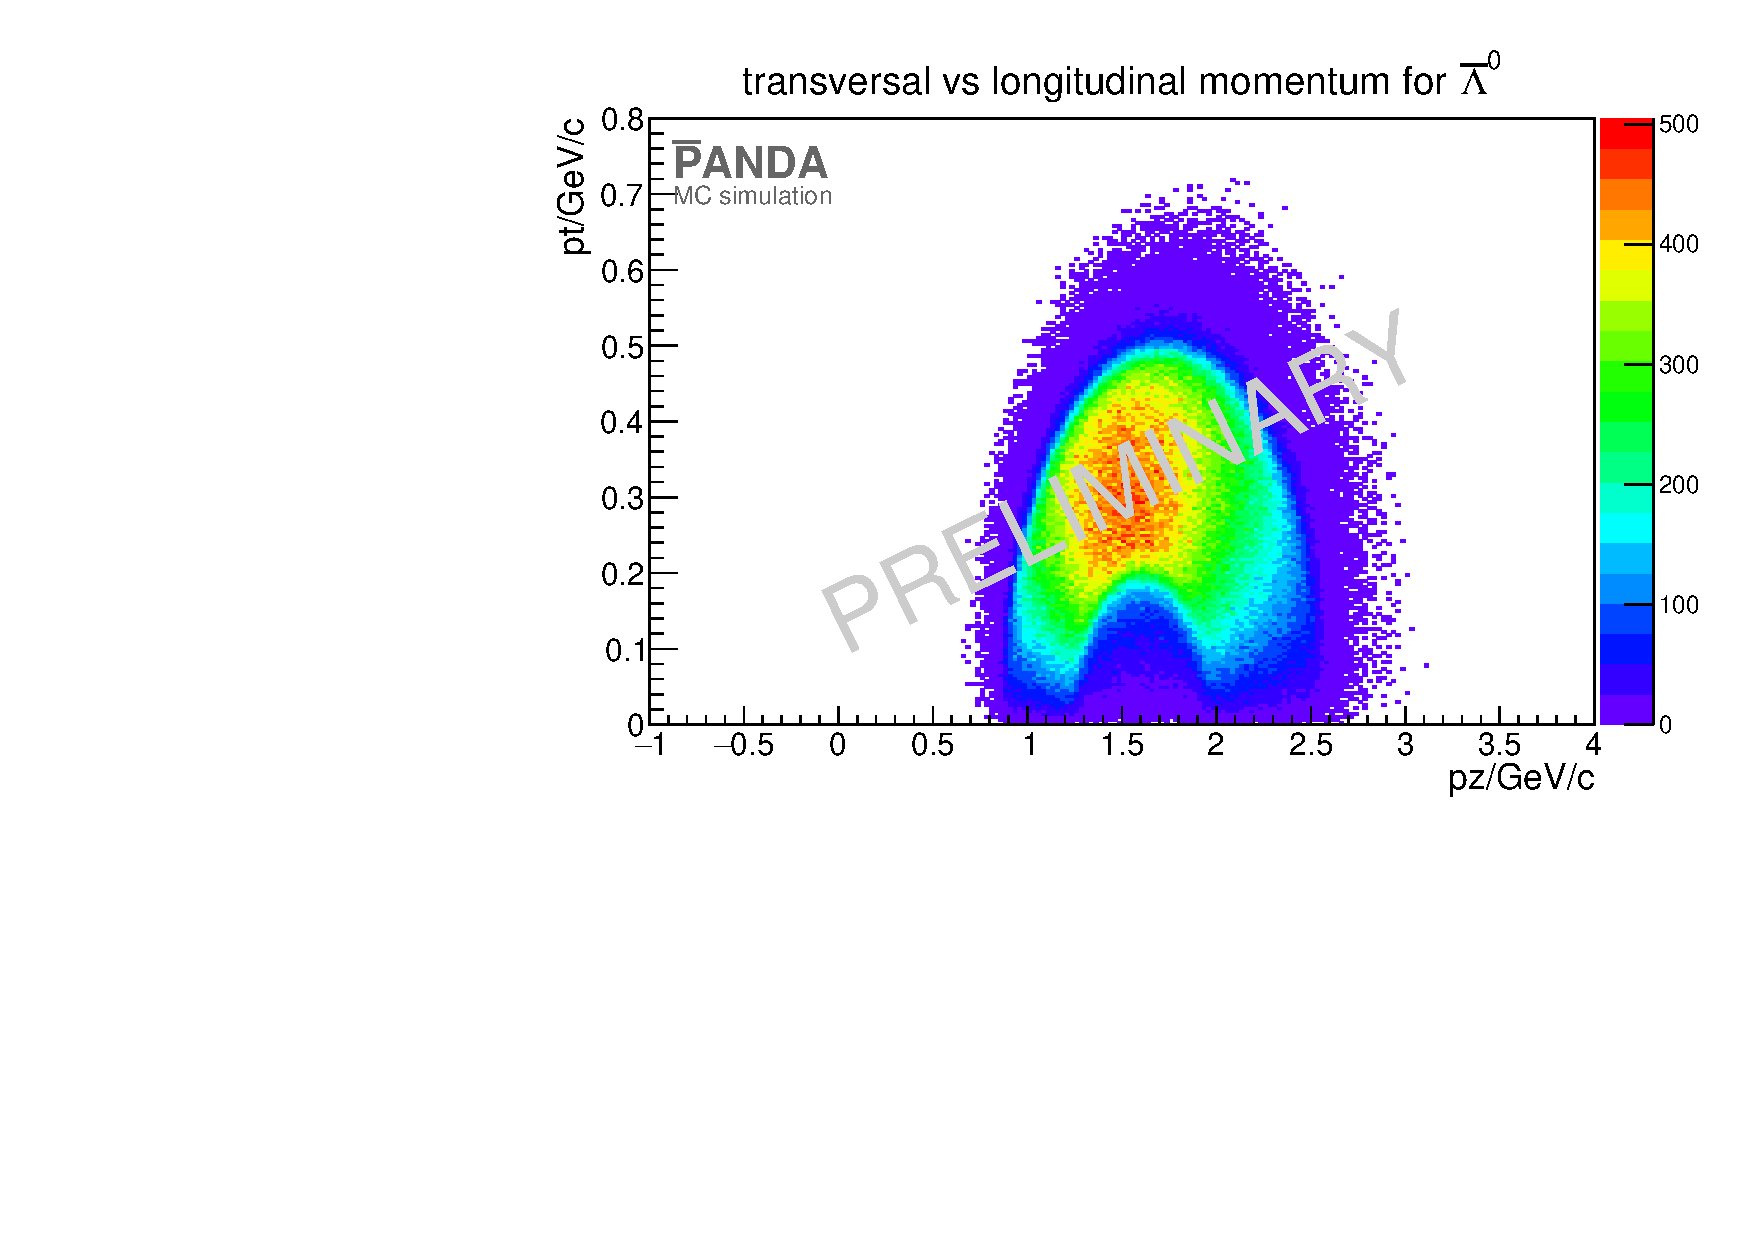
\includegraphics[width=0.49\textwidth]{./plots/antilambda0/AntiLambda0_MC_pt_vs_pz.pdf}}
	\caption{Figure a) shows transversal against the longitudinal momentum distribution for \lam. Figure b) 
			transversal versus longitudinal momentum distribution for \alam.}
	\label{fig:MC_lambda0_pt_vs_pz}
\end{figure}


\begin{figure}
	\subfigure[\anticascade]{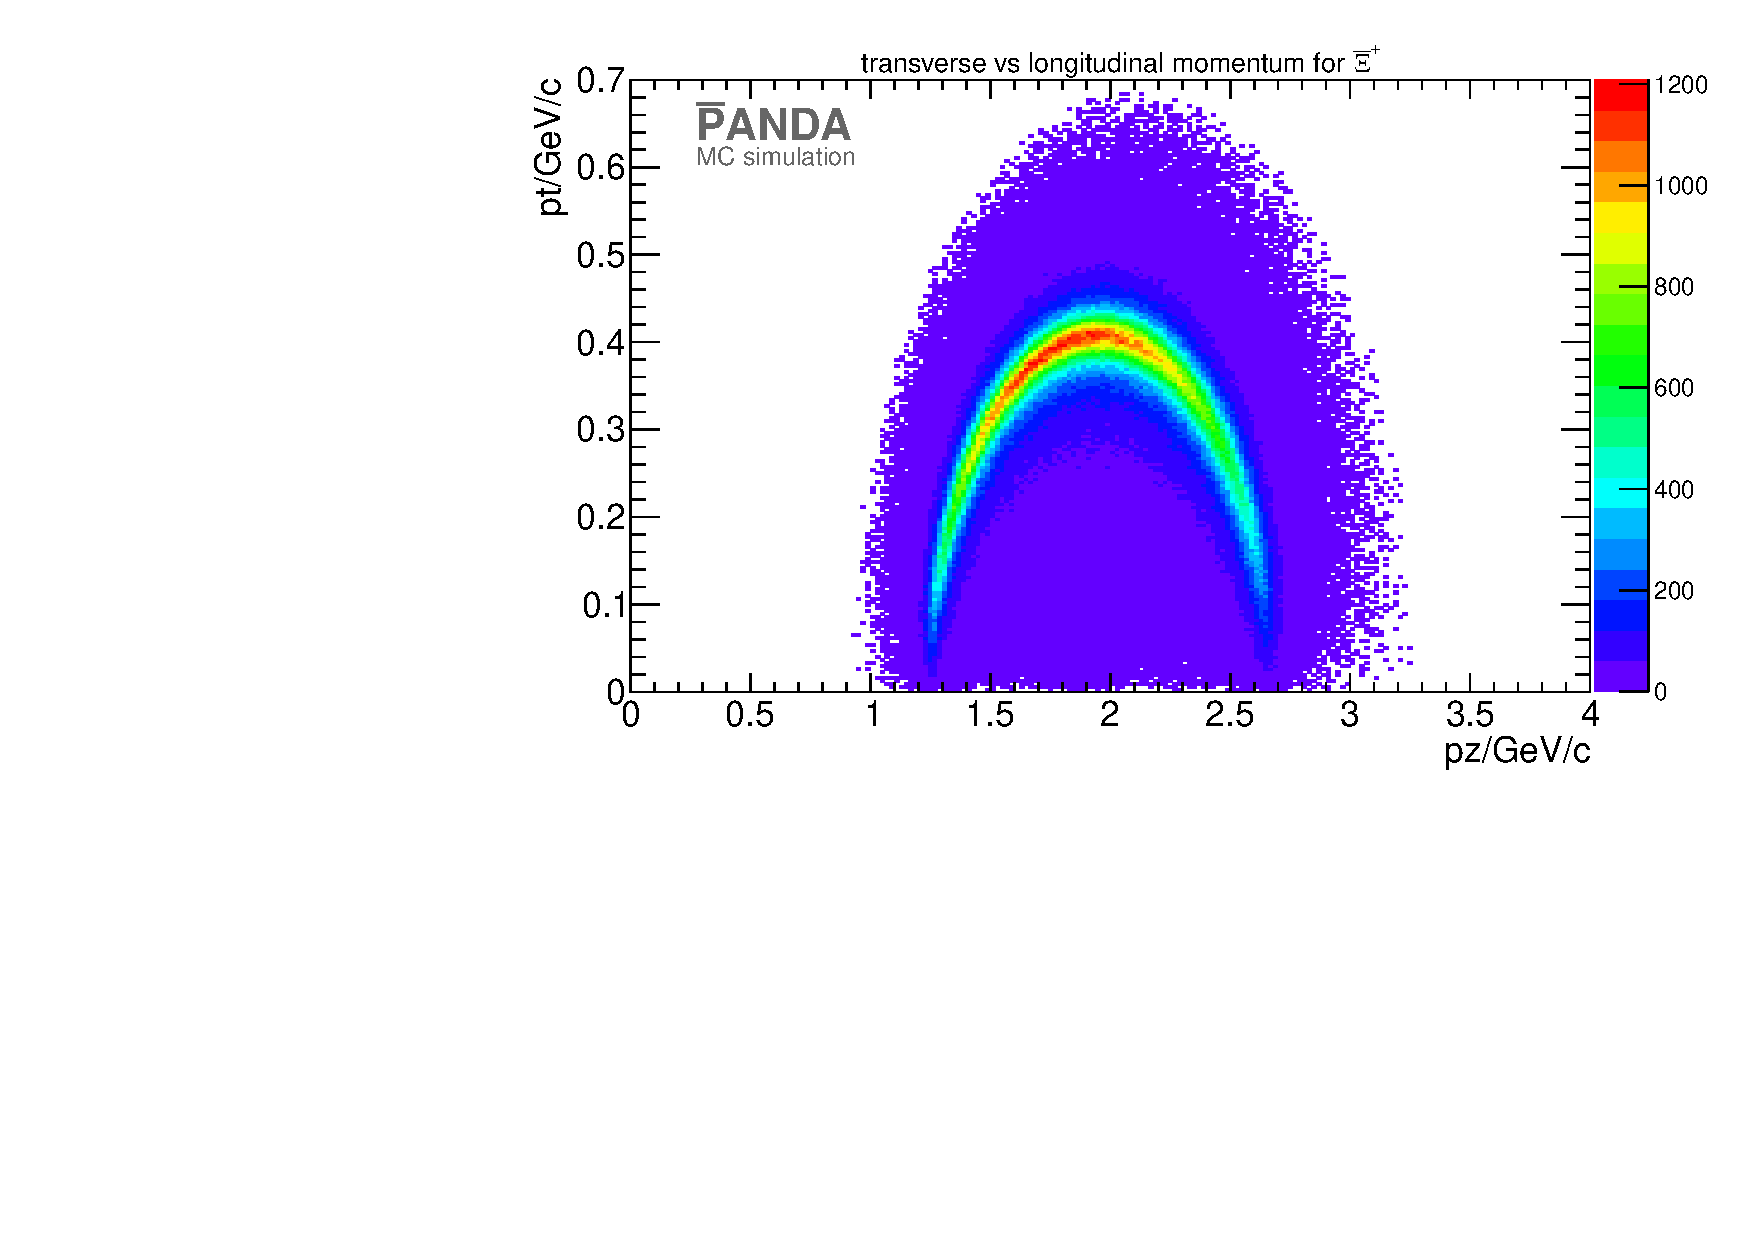
\includegraphics[width=0.49\textwidth]{./plots/Xi/XiPlus_MC_pt_vs_pz.pdf}}
	\subfigure[\excitedcascade]{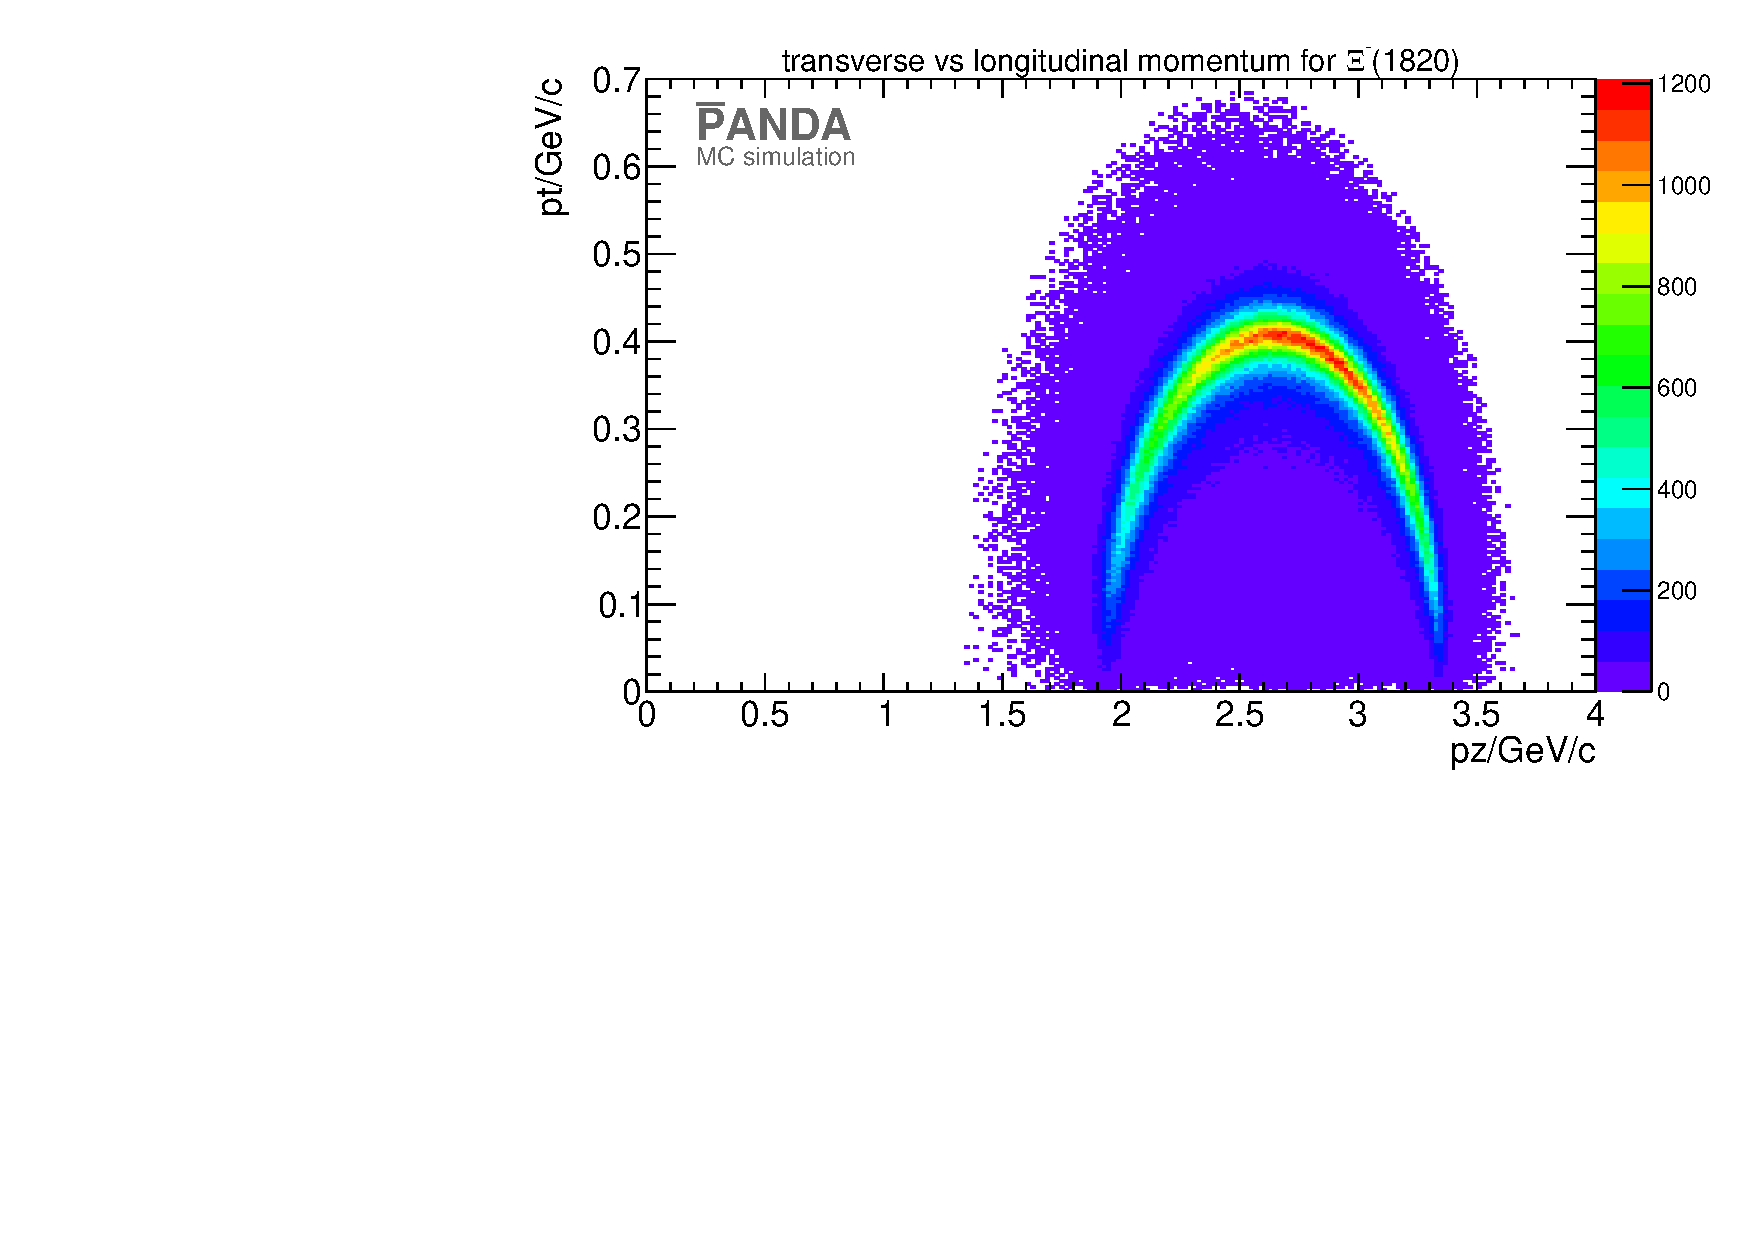
\includegraphics[width=0.49\textwidth]{./plots/Xi1820/XiMinus1820_MC_pt_vs_pz.pdf}}
	\caption{Figure a) shows transversal against the longitudinal momentum distribution for \anticascade. Figure b) 
			transversal versus longitudinal momentum distribution for \excitedcascade.}
	\label{fig:MC_xi_pt_vs_pz}
\end{figure}

Figure \ref{fig:eventgeneration_dalitz} shows the Dalitz plot for the \lam, \kminus and \anticascade final states for 
the channel \pbarpSystem $\rightarrow$ \excitedcascade \anticascade. 

\begin{figure}
	\centering
	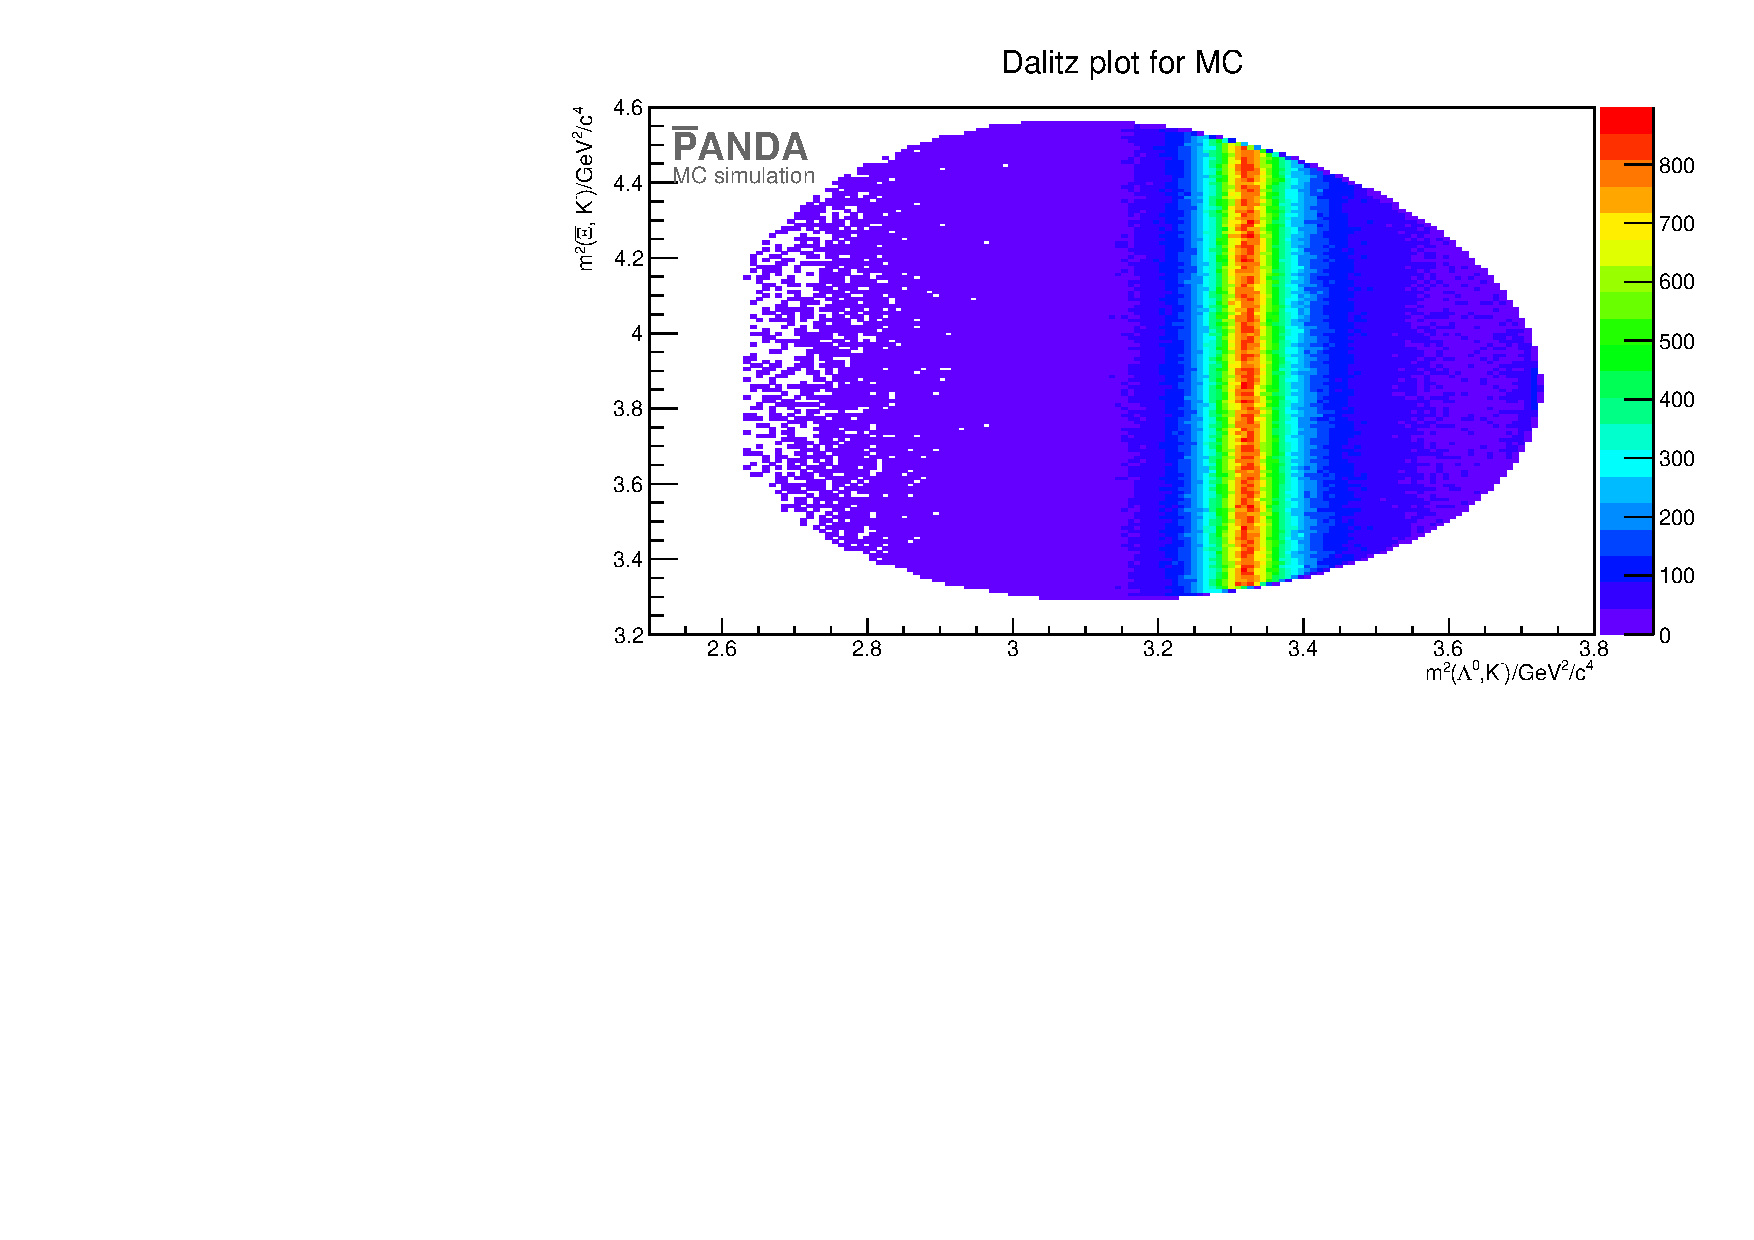
\includegraphics[width=0.6\textwidth]{./plots/Dalitzplot_MC.pdf}
	\caption{Dalitz plot for simulation. On x axis is the mass square of \lam  and \kminus and on the y axis there is the mass square of \anticascade and \kminus}
	\label{fig:eventgeneration_dalitz}
\end{figure}

